\documentclass{article}
\usepackage[margin=1in]{geometry}
\usepackage{graphicx}
\usepackage{amsthm}
\usepackage{enumitem}
\usepackage{amsmath}
\usepackage{amsfonts}
\setlength{\parindent}{0 pt}
\setlength{\parskip}{1 em}
\title{Differential Geometry Class Notes}
\author{Tim Player }
\date{September 16 2019}



\begin{document}

\maketitle

\section{Regular Curves}
Overview of key concepts will be covered in today's lecture.
\underline{Definition}
A \emph{parametrized differentiable curve} is a differentiable map $\alpha : I \to \mathbb{R}^n$ of an open
interval $I = (a,b)$ of the real line $\mathbb{R}$ into $\mathbb{R}^n$. \\
\underline{Limitations of multivaraible functions for complex shapes:}
As we learned in 8th grade a function can return only one value for each input. This means that certain shapes are not possible. We see this visually with the vertical line test test. \\
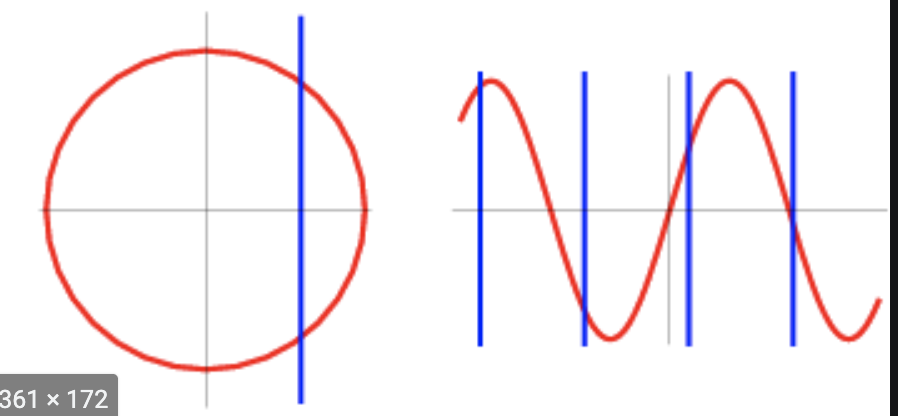
\includegraphics[scale=.5]{vline.png} \\
But a circle can be modeled easily with a parametric curve. Use $I = (0, 2\pi), \alpha(t) = (cos(t), sin(t))$\\
\underline{Definition} \textit{Regular curves} are curves where at least the second derivative exists and $\alpha'(t) \ne 0$. These are curves to which you can fit data.
\Remark {we require  $\alpha'(t) \ne 0$ to guarantee the existence of tangent vectors. Later we also require $\alpha''(t) \ne 0$ to guarantee the existence of normal vectors.} \\

\begin{itemize}
    \item $x^2 + y^2 = 1$
    \item $\alpha(t) = (\cos(t), \sin(t))$
    \item $\begin{cases}
        x = \sin(t) \\
        y = \cos(t) , 0 < t <= 2\pi 
        \end{cases}$
    \item $\beta(t) = e^{i t}$
\end{itemize}
Note: The second is a parametrized curve. Also the second and third have different orientations. 
The first one, does not tell us any orientations. 

Let's see another example. A helix in $\mathbb{R}^3$.
The parametrized helix can be written as a 3D curve 
\[
\gamma(t) = (\cos(t), \sin(t), t)
\]
When the curve is parameterized by \textit{arc length} (i.e., speed at each point is 1), then we can use the Frenet Frame to describe the curve locally. You can think of this as a three-arrowed axis which travels along the curve and describes the rate change of these frames along the curve. 

\textbf{Recall:} a function being differentiable can be tested by looking at whether
\begin{align*}
    \frac{\partial f_i}{\partial{x_j}}
\end{align*}
exists and is continuous for all $i$ and $j$ (This is called $C^1$ differentiable). This is  a sufficient condition for $f$ being $C^1$ differentiable. However, when we speak of parameterized curves being ``differentiable", we really mean smooth or infinitely differentiable, i.e. $f \in \mathbb{C}^\infty$

Recall: a function $f \colon \mathbb{R}^n \to \mathbb{R}^m$ is differentiable only if each of its $m$ component functions is differentiable.

\textbf{Example} Helix:
$x^2 + y^2 = a^2$ in $\mathbb{R}^3$, such that $z$ can be anything. Observe that this function, in $\mathbb{R}^2,$ is a circle. 

We may parameterize the circle as 
\[
\begin{cases}
        x(t) = a\cos(t) \\
        y(t) = a\sin(t)  
\end{cases}
0 < t <= 2\pi 
\]

which implies the parametrized curve being
\begin{align*}
    \alpha(t) = (a \cos(t), a \sin(t))
\end{align*}

The following is a different parametrized curve even they have the same trace. 
\[
\begin{cases}
        x = \sin(t) \\
        y = \cos(t)  
\end{cases}
0 < t <= 2\pi 
\]

which implies the parametrized curve is
\begin{align*}
    \beta(t) = (a \sin(t), a \cos(t))
\end{align*}

for the parameter 
$0 < t <= 2\pi.$

Consider another parametrized curve, which have same trace
\[
\begin{cases}
        x = \cos(2 \pi t) \\
        y = \sin(2 \pi t)  
\end{cases}
0 < t <= 1 
\]
Which may be written as 
\begin{align*}
    \gamma(t) = (a \cos(2 \pi t), a \sin(2 \pi t))
\end{align*}


These parameterizations trace out the same curve and we say that they have the same \textit{trace}.
Q: why do we need to use parametrized curve? \\
A: Let's understand the reason by above examples.  A parametrized curve describes a curve as a particle, it records the moving particle orientations, even back and forth motion in the middle of a circle or a motion cover the circle many times. But $x^2 + y^2 =1$ is after the "battle", just leaving us a trace.  Therefore parametrized curves can capture dynamics and kinematics in physics and computer vision (e.g. see a person moving forward then backward on pedestrian walkways.)

Consider the magnitude of the derivative of the first parameterization.
We find that 
\begin{align*}
    ||\alpha'(t)|| &= \sqrt{(-a \sin(t))^2 + (a \cos(t))^2}\\
    &= \sqrt{a^2(\sin^2t + \cos^2(t))}\\
    &= \sqrt{a^2}\\
    &= a.
\end{align*}

For the other parameterization, $\gamma$, we find that 
\begin{align*}
    \gamma'(t) &= (-2 \pi a \sin( 2 \pi t), 2 \pi a \cos( 2 \pi t)\\
    ||\gamma'(t)||&= \sqrt{(-2 \pi a)^2(\sin^2t + \cos^2(t))}\\
    &= 2 \pi a.
\end{align*}

Example 3.
\begin{align*}
    \alpha \colon \mathbb{R} \to \mathbb{R}^2 \\
    t \to (t^3, t^2) = \alpha(t)\\
    \alpha'(t) = (3t^2, 2t) = \vec{0} \\
    \begin{cases}
            3t^2 = 0\\
            2t = 0
    \end{cases}
    t=0
\end{align*}
$\alpha$ at t=0 is not regular.

Example 4.
\begin{align*}
    \alpha \colon \mathbb{R} \to \mathbb{R}^2 \\
    t \to (t^3 - 4t, t^2 - 4) = \alpha(t)\\
    \alpha'(t) = (3t^2-4, 2t) = \vec{0} \Longleftrightarrow
        \begin{cases}
            3t^2-4 = 0\\
            2t = 0
    \end{cases}
    t=0, -4 \ne 0.
\end{align*}
Every point is regular.

Example 5. See the slides.
Example 6.
Find the intersection curve in a parametric form of sphere $x^2 + y^2 + z^2 = 2^2$ and cylinder $(x - 1)^2 + y^2 = 1.$
This will be our homework!

Solution:
Hint: Let
\[
\begin{cases}
        x-1 = \cos(t) \\
        y = \sin(t) \\
        z = s
\end{cases}
\]
Then, plug this set of equations into the equation of the sphere. You get
\[
(1 + \cos(t))^2 + \sin(t)^2 + s^2 = 4.
\]
Then you can solve for $s$ in terms of $t$. This is called a Viviani curve. If you want to find the lenth of this curve, them the length formula is non-integrable. Our homework will be to find a parametrization of this curve, and approximate the length of this curve use numerical method.

\section{Arc Length of a Curve}
\textbf{Definition.} Arc length. Refer to handout.
Example: consider the circle
$$\alpha(t) = (\cos(t), \sin(t)),$$
where $0 \le t \le 2\pi$. Equivalently, consider 
$$\beta(t) = (\cos(2\pi t), \sin(2 \pi t)),$$ where $t \in [0, 1]$

\textbf{Definition.} $\alpha$ is parameterized by arc length if an only if it has unit speed.

In the above example, $\alpha$ is parameterized by arc length but $\beta$ is not.  That is since 
\begin{align*}
    \alpha'(t) &= (-\sin(t), \cos(t))\\
    ||\alpha'(t)|| &= 1
\end{align*}
while
\begin{align*}
    \beta'(t) &= (-2 \pi \sin(t), 2 \pi \cos(t))\\
    ||\beta'(t)|| &= 2\pi &(\text{which is not 1}).
\end{align*}

Why do we need a curve parameterized by arc length? Here is why. 
\begin{align*}
    \alpha(s) \tag{parameterized by arc length}\\
    ||\alpha'(s)|| = 1 \\
    ||\alpha'(s)||^2 = 1 \\
    \alpha'(s) \cdot \alpha'(s) = 1
\end{align*}
When you take the derivative of both sides, you get 
\begin{align*}
     \alpha''(s) \cdot \alpha'(s) +  \alpha'(s) \cdot \alpha''(s) &= 0 \\
     2(\alpha''(s) \cdot \alpha'(s)) = 0 \\
     \alpha''(s) \perp \alpha'(s)
\end{align*}
Which shows that the second derivative of $\alpha$ is guaranteed to be orthogonal to its velocity if it is parameterized by arc length. This has applications to the Frenet Frame.

\textbf{Definition.} Frenet Frame. With $||\alpha'(s)|| = 1,$ let $\vec{t} =\alpha'(s)$ be the tangent vector. Then, let 
\[
\vec{n} = \frac{\alpha''(s)}{||\alpha''(s)||}.
\]

Define $\vec{b} = \vec{t} \times \vec{n}$.  Now $\{\vec{t}, \vec{n}, \vec{b}\}$ forms the Frenet Frame, which is an orthonormal frame.

Now taking the derivative of $\vec{b} = \vec{t} \times \vec{n}$, you get torsion,
Here is some work showing that.

\begin{align*}
    \vec{b}(s) = \vec{t}(s) \times \vec{n}(s).
\end{align*}
Claim: 
\begin{align*}
    \vec{b}'(s) = \tau(s) \vec{n}(s).
\end{align*}
Proof:
Key idea: we prove $\vec{b}'(s) \perp \vec{t}(s)$ and $\vec{b}'(s) \perp \vec{b}(s);$ which will force $\vec{b}'(s) \paralell \vec{n}(s)$

We start with 
\begin{align*}
    \vec{b}(s) = \vec{t}(s) \times \vec{n}(s).
\end{align*}

We take the derivative of both sides to get 
\begin{align*}
    \vec{b}'(s) = vec{t}'(s)\ \times \vec{n}(s) + \vec{t}(s) \times \vec{n}'(s)
\end{align*}
The left term of the RHS is zero since $\vec{t}'(s)$ is $\vec{n}(s)$ , which implies that $\vec{b}''(s) \perp \vec{t}(s)$.

To prove the second claim, we again start with 
\begin{align*}
    \vec{b}(s) &= \vec{t}(s) \times \vec{n}(s)\\
    ||\vec{b}(s)|| &= ||\vec{t}(s) \times \vec{n}(s)||\\
    &= ||\vec{t}(s)|| \, ||\vec{n}(s)|| \sin\theta\\
    &= 1
\end{align*}
Having shown that, we note the implication that
\begin{align*}
    ||\vec{b}(s)||^2 &= 1\\
    \vec{b}(s) \cdot \vec{b}(s) &= 1 \tag{Now take the derivative.}\\
    \vec{b}'(s) \cdot \vec{b}(s) + \vec{b}(s) \cdot \vec{b}'(s)&= 0 \\
    2 \vec{b}'(s) \cdot \vec{b}(s) &= 0 \\
    \vec{b}'(s) \perp \vec{b}(s)
\end{align*}

Note that $\alpha''(s) = (\alpha'(s))'$. That is you can interpret the second derivative of a curve $\alpha$ as the rate of change of its tangent vectors.

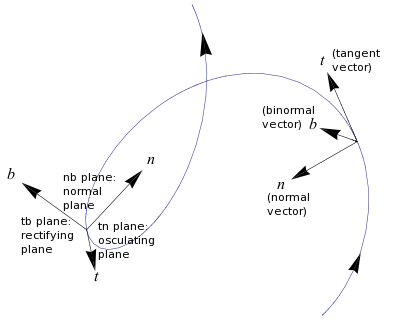
\includegraphics[scale=.9]{FrenetFrame.png}

\underline{Definition} The speed is $\tau(s)$ \\
\textbf{Definition} Curvature. 
\begin{defn}
Let $\alpha : I \to \R^3$ be a curve parametrized by arc length $s \in I$. The number $\|\alpha''(s) \|
= k(s)$ is called the \emph{curvature} of $\alpha$ at $s$.
\end{defn} \\
\underline{Geometric Meaning}
Let $\alpha : I = (a,b) \to \R^3$ be a curve parametrized by arc length $s$. Since the tangent
vector $\alpha'(s)$ has unit length, the norm $\| \alpha''(s) \|$ of the second derivative measures the
rate of change of the angle which neighboring tangents make with the tangent at $s$.
$\| \alpha''(s) \|$ gives, therefore, a measure of how rapidly the curve pulls away from the tangent
line at $s$, in a neighborhood of $s$.

Another geometric meaning: Curvature is related to the radius of the circle most closely fitting a curve at a point, such that $K =\frac{1}{R}.$ \\
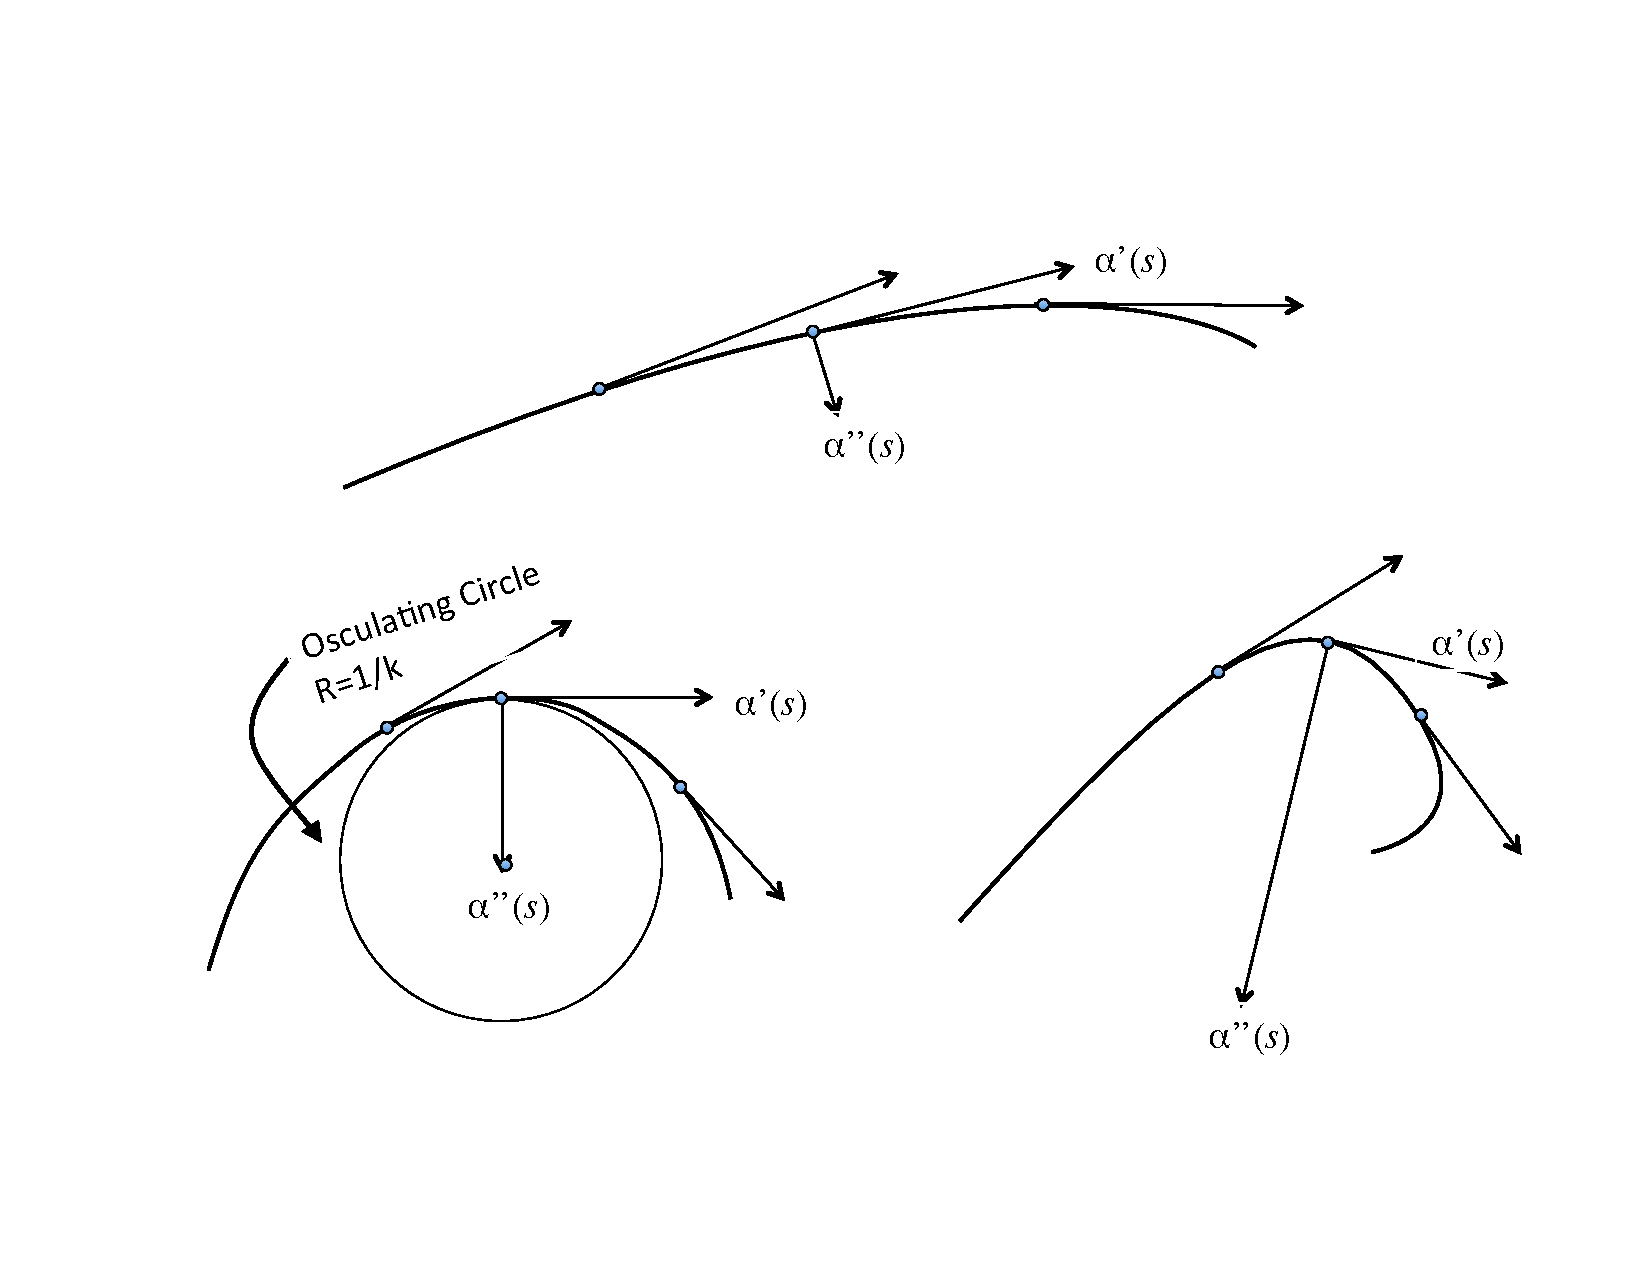
\includegraphics[scale=.4]{curvature.pdf}\\
\underline{Torsion}
Since $b(s)$ is a unit vector, the length $\|b'(s)\|$ measures the rate of change of the neighboring
osculating planes with the osculating plane at $s$; that is $b'(s)$ measures how rapidly the curve
pulls away from the osculating plane at $s$, in a neighborhood of $s$. \\
\begin{center} 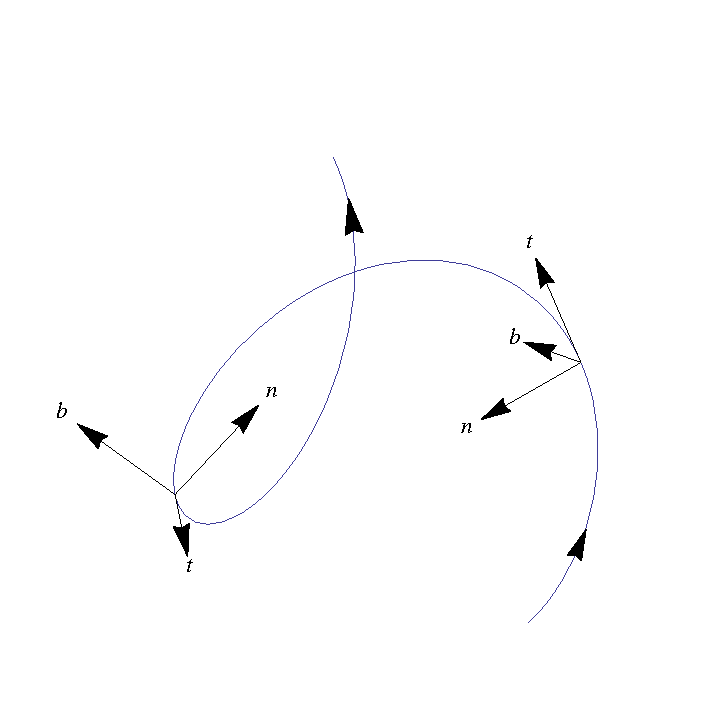
\includegraphics[scale=0.6]{torsion.pdf} \end{center}
Let $\alpha : I \to \R^3$ be a curve parametrized by arc length $s$ such that $\alpha''(s) \ne 0,
s \in I$. The number $\tau(s)$ defined by $\vec{b}'(s) = \tau(s) \vec{n}(s)$ is called the
\emph{torsion} of $\alpha$ at $s$.


\section{Frenet Formula}
\begin{align*}
    \begin{cases}
            \vec{t}'(s) &= 0\vec{t}(s) +k(s) \vec{n}(s) + 0\vec{b}(s) \\
            \vec{n}'(s) &= -k(s)\vec{t}(s) + 0 \vec{n}(s) + \tau(s) \\
            \vec{b}'(s) &= 0 \vec{t}(s) + \tau(s) \vec{n}(s) + 0 \vec{b}(s) \\
    \end{cases}
\end{align*}

Let's figure out what is $\vec{n}'(s)$. 

\begin{align*}
    \vec{n}(s) &= b(s) \times t(s) \\
    \vec{n}'(s) &= b'(s) \times t(s) + b(s) \times t'(s) \\
    &= \tau(s) \vec{n}(s) \times \vec{t}(s) + \vec{b} \times k(s) \vec{n}(s)\\
    &=- \tau(s)\vec{b}(s) - k(s) \vec{t}(s)
\end{align*}

This exercise has shown us that we can fill in the matrix
\begin{align*}
    \begin{bmatrix}
        \vec{t}'(s) \\
        \vec{n}'(s)\\
        \vec{b}'(s)
    \end{bmatrix}
    = 
    \begin{bmatrix}
        0 &k(s) &0\\
        -k(s) &0 &-\tau(s)\\
        0 &\tau(s) &0
    \end{bmatrix}
    \begin{bmatrix}
        \vec{t}(s) \\
        \vec{n}(s)\\
        \vec{b}(s)
    \end{bmatrix}
\end{align*}
called the Frenet Formula. 

This is important because it theoretically gives us a key new method to study curved objects (such as manifolds!) by using a linear algebra problem.

For instance, consider a surface

\begin{align*}
    \mathbf{X}(u,v) = (x(u, v), y(u,v), z(u,v)),
\end{align*}

this could be the sphere $x^2 + y^2 + z^2 = 1,$ with parameterization
\begin{align*}
    \mathbf{X}(u,v) = (\cos u \cos v, \sin u \cos v, \sin v).
\end{align*}

Using Frenet's Formula, you can examine the behavior local to any point.

This can be applied to applications such as 
\begin{itemize}
    \item identifying anomalous behavior from UAVs
    \item determining the trajectory of a cell phone using the onboard sensor data, and using the trajectory to analyze gait and identify users
    \item robotic surgery
\end{itemize}

\section{Local Canonical Form for Curves}
Local canoncical form is an approximation. You get it by taylor expanding around a single point. 
Consider any curve $\alpha(s)$. Let's expand around $0$.
\begin{align*}
    \alpha(s) &= \alpha(0) + s \alpha'(0) + \frac{s^2}{2!}\alpha''(0) + \frac{s^3}{3!}\alpha'''(0) + \cdots \\ && \text{$\alpha(0)$, $\alpha'(0)$ and the others are vectors obtained by expanding termwise}\\
    &= (x(s), y(s), z(s) \tag*{Now, Taylor expand each dimension.}\\
    &= (x(0) + x'(0)t + \frac{1}{2!}x''(0)t^2 + \hdots \;\;y(0) + y'(0)t + \frac{1}{2!}y''(0)t^2 + \hdots \;\; z(0) + z'(0)t + \frac{1}{2!}z''(0)t^2 + \hdots)\\
    &= 
    \begin{pmatrix}
    x(0)\\
    y(0)\\
    z(0)
    \end{pmatrix}
    +
    \begin{pmatrix}
    x'(0)\\
    y'(0)\\
    z'(0)
    \end{pmatrix}
    t + \hdots
\end{align*}

Recall now that
\begin{align*}
    \alpha'''(s) &= (\alpha''(s))'\\
    &=(k(s) \vec{n}s)'\\
    &=k'(s)\vec{n}(s) + \vec{n}'(s)k(s) \\
    &=k'(s)\vec{n}(s) + (-k\vec{t} - \tau \vec{b})k(s)
\end{align*}

We can similarly investigate the other terms of the Taylor expansion. We use 
\begin{align*}
    \alpha'(s) = \vec{t}(s)\\
    \alpha''(s) = k(s)\vec{n}(s)\\
    \alpha'''(s) = k'(s)\vec{n}(s) + (-k\vec{t} - \tau \vec{b})k(s)
\end{align*}
Let $R$ be the remainder after expanding to 4 terms.
which allows us to collect
\begin{align*}
    \alpha(s) - \alpha(0) = \left[ s - \frac{s^3}{3!}k^2(s)\right]\tau(s) +
    \left[\frac{s^s}{2!}k(s) +  \frac{s^3}{3!}k'(s)\right]\vec{n}(s) +
    \left[\frac{s^3}{3!}\tau(s)k(s)\right]\vec{b}(s) + \vec{R}
\end{align*}
which gives us a local representation of the curve, called Local Canonical Form.
\begin{align*}
    x(s) &= s - \frac{s^3}{3!}k^2(s) + R_x \\
    y(s) &= \frac{k}{2}s^2 + \frac{s^3}{3!}k'(s) + R_y \\
    z(s) &= -\frac{k\tau}{3!}s^3 + R_z
\end{align*}
\end{document}

